%\addcontentsline{toc}{section}{Propuesta de soluci\'on}
%\section*{Propuesta de soluci\'on}
%\addcontentsline{toc}{subsection}{Definición de la metodología}
\subsection{Marco Precedimental}

\subsubsection{Definici\'on de la metodolog\'ia mecatr\'onica}

La mecatrónica es una ingeniería interdisciplinaria y, por tanto, es necesario buscar 
metodologías de diseño que nos permita especificar las necesidades del sistema, planear actividades, dividir tareas y validar resultados.
\\
En \cite{Geusemeir2002} se muestra la metodología mecatrónica ‘VDI 2206”. En ella se sigue un modelo 
procedimental flexible basado en tres elementos principales:
\begin{itemize}
    \item El ciclo general de resolución de problemas a pequeña escala (micro-level)
    \item El modelo en forma de V en la gran escala (macro-level)
    \item Módulo de procesos predefinidos para pasos de operación que se repiten durante el diseño de los sistemas mecatrónicos.
\end{itemize}

\subsubsection{Resolución de problemas en el micro-level}
La resolución de problemas en el micro-level comienza de dos maneras: analizando la situación actual y analizando la relación de la condición actual con la condición meta. Lo anterior nos lleva a una síntesis y análisis que permite generar, rechazar y elegir soluciones. El análisis de la solución y la evaluación nos puede llevar a replantear la meta o a volver a analizar la situación. Si el resultado es satisfactorio nos sirve como herramienta de aprendizaje y se planean las acciones futuras. \\
El flujo de esta metodología de resolución de problemas se puede ver en la figura \ref{fig:DiagramaMicroLevel}:
%---------------------------------Imagen 3---------------------------------
\begin{figure}[!htb]
    \centering
    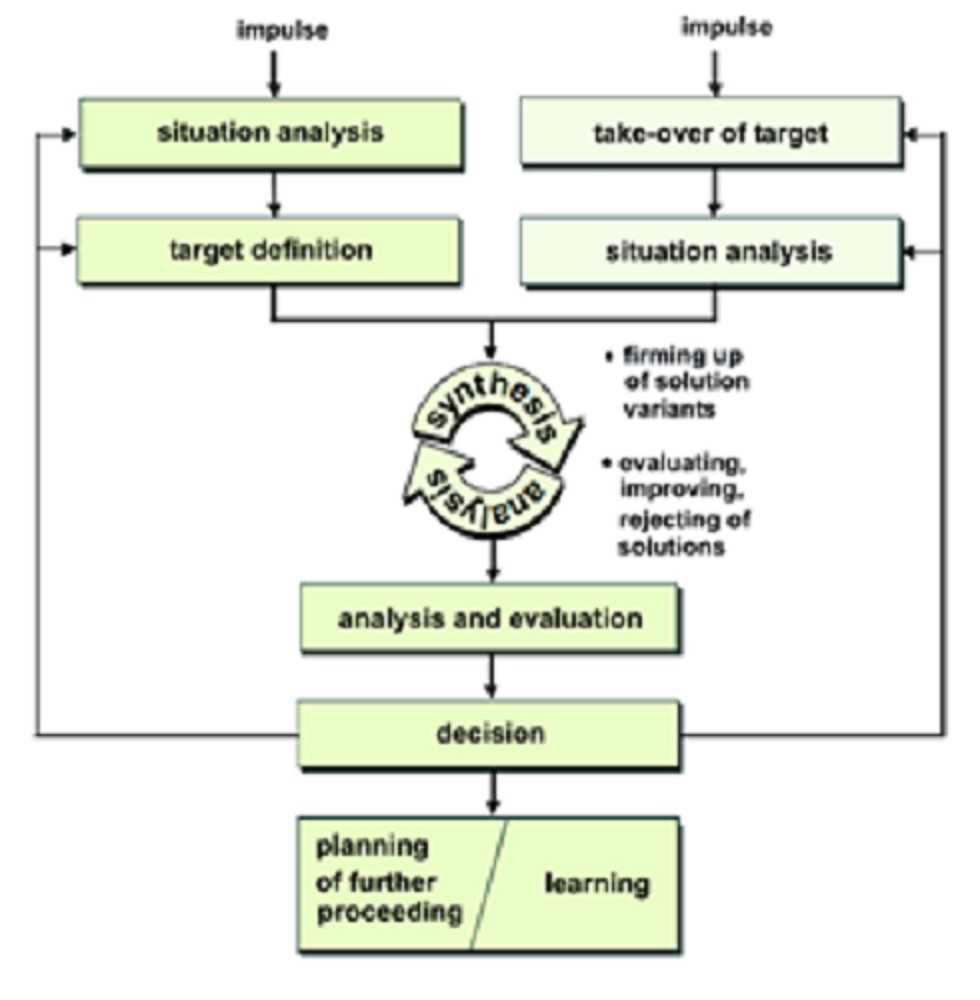
\includegraphics[width=0.6\textwidth]{imagenes/3.jpg}
    \caption{Diagrama de flujo para la resolución de problemas en el micro-level.}
    \label{fig:DiagramaMicroLevel}
\end{figure}
\FloatBarrier
%---------------------------------Imagen 3---------------------------------

\subsubsection{Modelo en V en el macro-level}
En modelo en V, en donde la primera parte es un procedimiento de arriba hacia abajo y la segunda parte es de abajo hacia arriba, nos permitirá separar las tareas a gran escala y realizar validaciones constantes de los sistemas.\\
El modelo V busca partir de los requerimientos y realizar un diseño del sistema conceptual, el cual es multidominio y describe las características esenciales del producto. A continuación, hace diseños específicos para cada dominio, los cuales integra en una etapa posterior y analiza sus interrelaciones. A lo largo de este proceso se debe hacer una verificación y validación constante de que el diseño cumpla con los requerimientos y el diseño conceptual del producto, además de apoyarse en el modelado y la simulación por computadora para hacer estas validaciones. En caso de cumplirse con esto se cuenta con un producto que cumple con los requisitos.\\
El modelo V es un modelo iterativo, es decir, es poco probable que el primer producto al que se llegue después de la integración sea totalmente funcional o incluso el óptimo. Por lo anterior, se deben llevar a cabo múltiples ciclos de diseño y validación, para que el producto alcance un mayor grado de madurez. Cada etapa tiene un “contraparte” a la que se puede volver en caso de que no se cumpla alguna verificación, esto lleva a mejorar el diseño y analizar múltiples opciones de solución.
%---------------------------------Imagen 4---------------------------------
\begin{figure}[!htb]
    \centering
    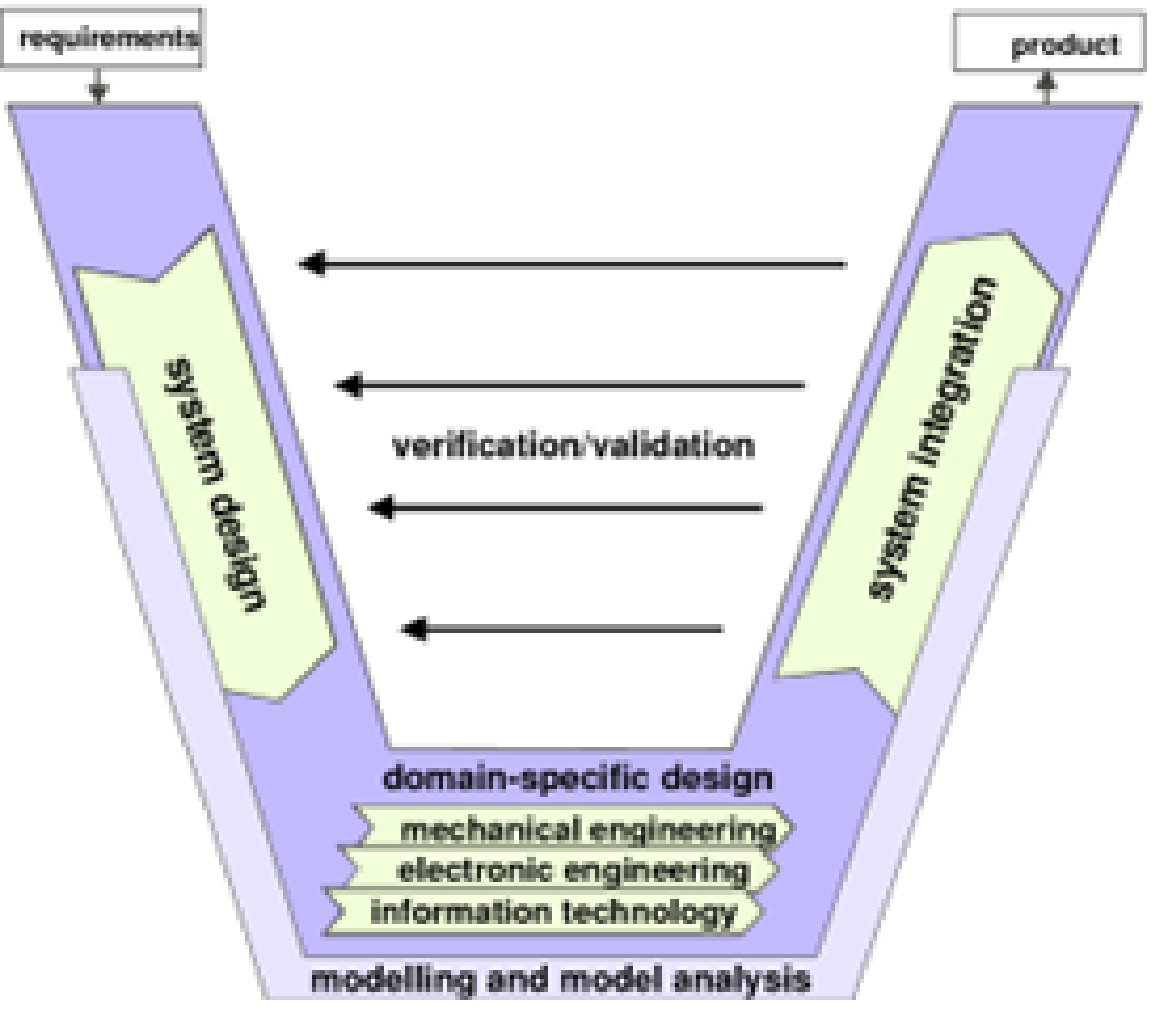
\includegraphics[width=0.5\textwidth]{imagenes/4.jpg}
    \caption{\footnotesize Metodología por seguir.}
    \label{Fig:MetodologiaV}
\end{figure}
\FloatBarrier
%---------------------------------Imagen 4---------------------------------

\subsubsection{Procesos predefinidos}
En cada una de las etapas de diseño, se tienen procesos predefinidos que se repiten regularmente durante estas etapas. Cada uno de estos procesos están mejor definidos en \cite{Pahl1996} y se utilizarán en el desarrollo de este proyecto para la generación de soluciones.